\chapter{Instalación y arranque del servidor Apache}
\section{Enunciado}
    5. Instalación y arranque del servidor Apache. Instalación de paquetes, ejecución de comandos de administración del servicio, etc. Revisión continua del fichero \texttt{error\_log} para detectar warnings y errores; y del \texttt{access\_log} para comprobar accesos.
\section{Resolución}
Se instalan los paquetes necesarios para el servidor web Apache y se habilita el módulo SSL para permitir conexiones seguras. Posteriormente, se reinicia el servicio para aplicar los cambios.
Comandos utilizados:
\begin{lstlisting}[language=bash]
sudo apt update
sudo apt install apache2
# Habilirar el módulo SSL
sudo a2enmod ssl
sudo systemctl restart apache2
\end{lstlisting}
Se comprueba el correcto funcionamiento del servidor accediendo a \href{https://www.ejemplo.com}{https://www.ejemplo.com} y revisando continuamente \texttt{/var/log/apache2/error\_log} para detectar *warnings* y errores; y \texttt{/var/log/apache2/access\_log} para comprobar accesos.
\begin{center}
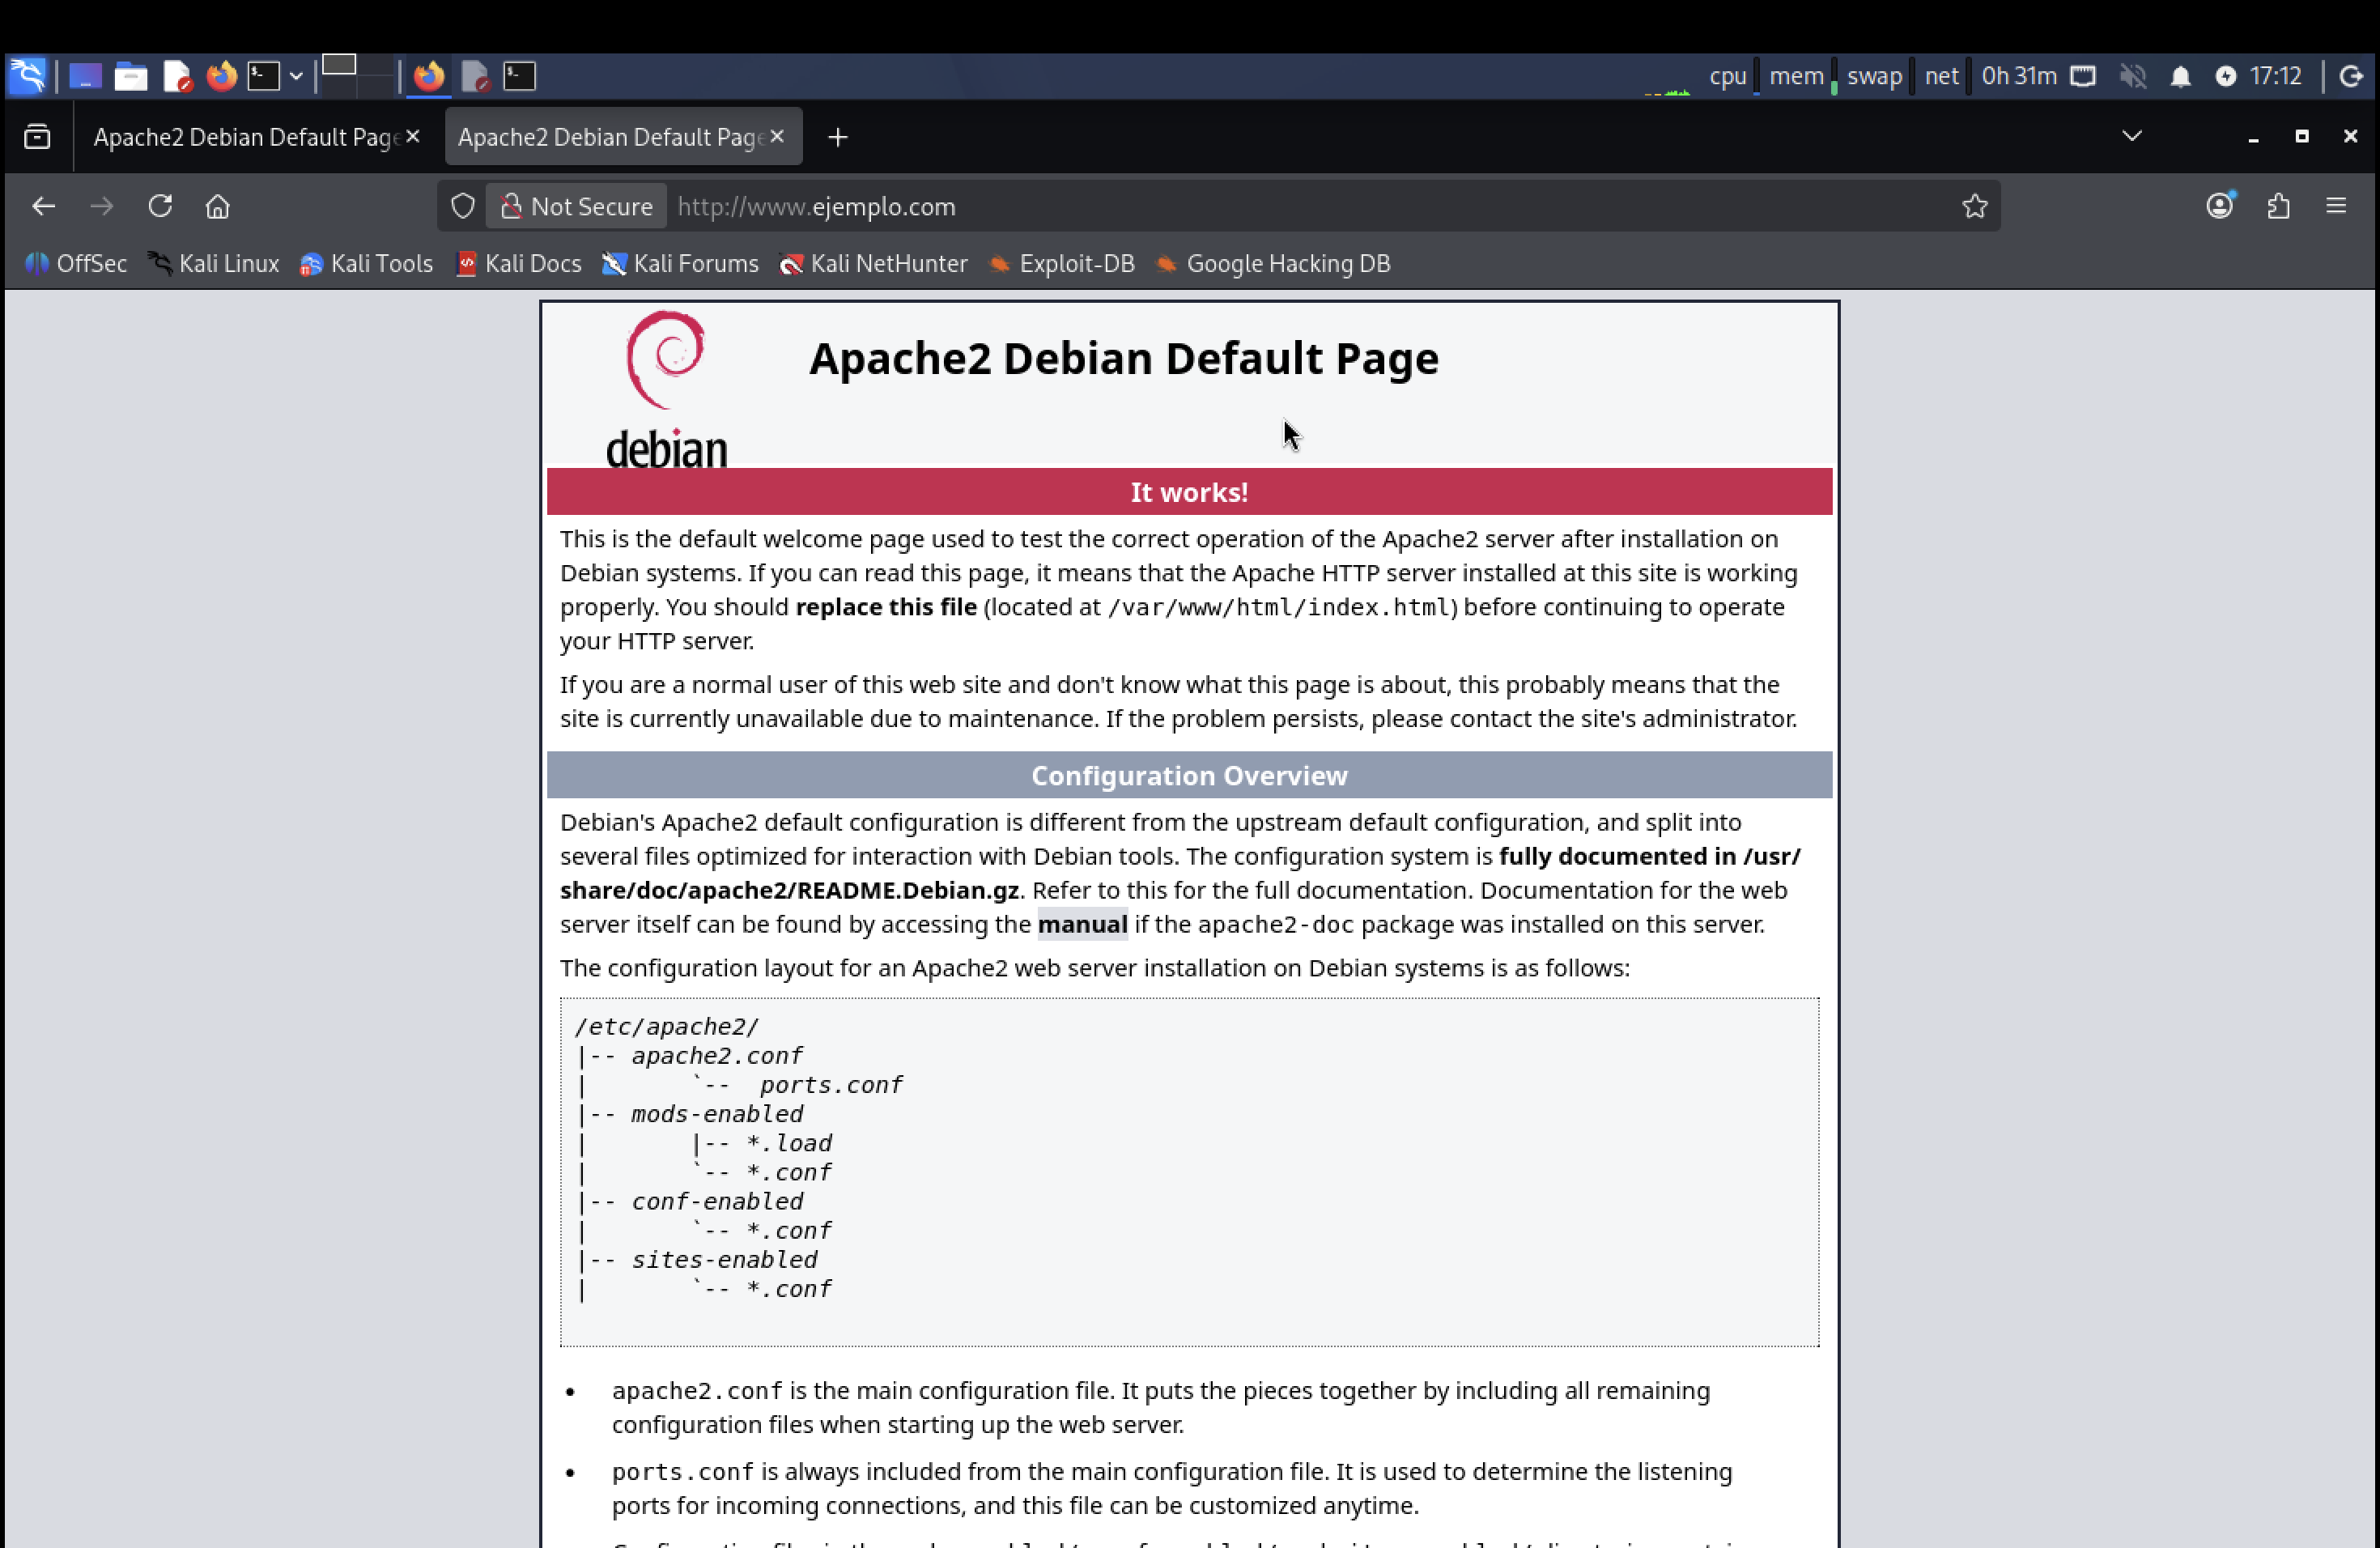
\includegraphics[width=0.9\textwidth]{Imagenes/2-default_apache_page.png}
\end{center}